\begin{center}
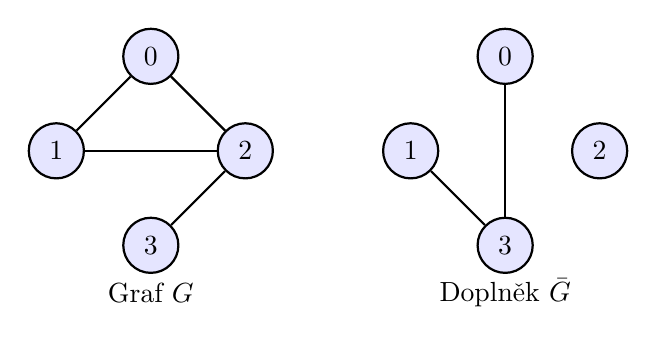
\begin{tikzpicture}[
  vnode/.style={circle, draw, minimum size=7mm, inner sep=0pt, fill=blue!10},
  thick
]
  \begin{scope}[shift={(0,0)}]
    \node[vnode] (0) at (0, 1.2) {0};
    \node[vnode] (1) at (-1.2, 0) {1};
    \node[vnode] (2) at (1.2, 0) {2};
    \node[vnode] (3) at (0, -1.2) {3};
    
    \draw (0) -- (1);
    \draw (0) -- (2);
    \draw (1) -- (2);
    \draw (2) -- (3);
    \node at (0, -1.8) {Graf $G$};
  \end{scope}
  
  \begin{scope}[shift={(4.5,0)}]
    \node[vnode] (0') at (0, 1.2) {0};
    \node[vnode] (1') at (-1.2, 0) {1};
    \node[vnode] (2') at (1.2, 0) {2};
    \node[vnode] (3') at (0, -1.2) {3};
    
    \draw (0') -- (3');
    \draw (1') -- (3');
    \node at (0, -1.8) {Doplněk $\bar{G}$};
  \end{scope}
\end{tikzpicture}
\par\medskip
\textit{Obrázek 3.4: Příklad grafu $G$ a jeho doplňku $\bar{G}$ na čtyřprvkové množině vrcholů.}
\end{center}